\documentclass[a4paper, 15pt]{article}
\usepackage[left=0.85in, right=0.85in, top=0.5in, bottom=0.95in]{geometry}
\usepackage[T1]{fontenc}
\usepackage[utf8]{inputenc}
\usepackage[italian]{babel}

% Formattazione del testo
\usepackage{setspace}         % Setting dello spazio\begin{spacing}{0.95}
\setstretch{1.2}
\setlength{\parindent}{0pt}
\raggedbottom
\usepackage[none]{hyphenat}    % no sillabazione 
\usepackage{multicol}          % testo su più colonne
\usepackage{changepage}	       % \begin{adjustwidth}{}{}

% Matematica
\usepackage{amsmath, amssymb, amsthm, mathtools}
\usepackage{cancel}            % semplificazioni \cancel{expression}
\newtheorem*{thm}{Teorema}
\newtheorem*{en}{Enunciato}
\newtheorem*{definizione}{Definizione}
\newtheorem*{cor}{Corollario}
\DeclareMathOperator{\rk}{rk}
\DeclareMathOperator{\im}{Im}
\DeclareMathOperator{\ev}{ev}

% Simboli e Disegni
\usepackage{color}             % \textcolor{'ColorCode'}{'testo'}
\usepackage{graphicx, wrapfig, float}
\usepackage{fancyhdr}
\usepackage{tikz, circuitikz}
\usetikzlibrary{patterns, arrows, decorations.markings, arrows.meta, decorations.text}
\tikzset{immagine/.style={above right, inner sep=0pt, outer sep=0pt},
testo/.style={fill=white, align=center, fill opacity=0.6, text opacity=1, below, font=\sffamily\bfseries\footnotesize}}
\usepackage{pgfplots}
\pgfplotsset{compat=1.15}
\usepackage{mathrsfs}

% Altri pacchetti
\usepackage{enumitem}
\usepackage{mdwlist} 	       % suspend enumerate \suspend{} \resume{}
\usepackage{siunitx}
\usepackage{hyperref}
\hypersetup{
colorlinks=true,
linkcolor=blue,    
urlcolor=blue,
}
\urlstyle{same}

% Altre definizioni personali
\usepackage{pifont}
\newcommand{\cmark}{\ding{51}}
\newcommand{\xmark}{\ding{55}}
\DeclareUnicodeCharacter{20AC}{\EUR}
\newcommand{\compresslist}{\setlength{\itemsep}{1pt}\setlength{\parskip}{0pt}\setlength{\parsep}{0pt}}
\newcommand{\ra}[1]{\renewcommand{\arraystretch}{#1}} % stretcho le tabelle e gli array \ra{x}
\setlength{\jot}{10pt}

%=======HEADER & FOOTER=======%
\def\lesson{Lezione N.28}


\pagestyle{fancy}
\fancyhf{}
\renewcommand{\headrulewidth}{0pt}
\renewcommand{\footrulewidth}{1.4pt}
\lfoot{A.M. $\diamond$ \the\year}
\cfoot{\thepage}
\rfoot{\lesson}


% Titolo e data
\title{Parte 20: resistenza degli ingranaggi}
\date{}

\begin{document}
\maketitle
\setcounterpageref{secnumdepth}{0}
\setcounter{tocdepth}{5}  % Includo nel TOC anche i subsubpar	
\tableofcontents 
\newpage



%\end{adjustwidth}
%\newpage
\section{Criteri di costruzione}
\begin{adjustwidth}{2in}{}
Prima di tutto, per verificare il corpo ruota, è necessario tenere in considerazione in posizionamento dell'ingranaggio sull'albero, questo infatti dev'essere verificato a resistenza e a rigidezza dovendo minimizzare gli spostamenti relativi. 

So dovrà fare così molta attenzione alla luce tra gli appoggio, cioè alla distanza tra i cuscinetti, così da minimizzare l'inflessione della trave appoggio-appoggio. 

Il rapporto tra la distanza dei cuscinetti ed il diametro dell'albero dovrebbe attestarsi intorno a valori di $2,5\div2,7$. 

Com'è noto, ridurre la distanza tra gli appoggi permette di limitare l'inflessione. 	\newline 

I materiali tipici da utilizzare per le ruote sono gli acciai a basso tenore di carbonio, leghe a base di nichel, facendo una distinzione tra ruote di pezzo e ruote calettate. \newline 

Altro aspetto da tenere in considerazione sarà la lubrificazione, così come per i cuscinetti, anche per gli ingranaggi si deve prevedere un sistema di lubrificazione, il più delle volte a bagno/nebbia d'olio. 

Il sistema di lubrificazione dev'essere tale da ridurre il carico termico dovuto all'attrito e garantire il coretto funzionamento attraverso uno smaltimento del calore ed il mantenimento della temperatura di \textit{bulk}, cioè la temperatura media degli elementi  intorno agli $80^\circ C$. 

Il lubrificate di base si attesta ad una temperatura tra i $(30\div40)^\circ C$, in prossimità dell'ingranaggio si riscalda e smaltisce il calore una volta allontanato.\newline 

La ruota dentata è sostanzialmente composta da tre parti:
\begin{enumerate}
	\item Una corona esterna, un disco dove vengono realizzati in denti.
	\item Un mozzo centrale, la parte di connessione con l'albero
	\item Un corpo ruota, la parte intermedia che connette il mozzo alla corona
\end{enumerate}  
Corona e mozzo solo elementi massivi, mentre invece il  corpo ruota può essere un elemento più leggero e sottile che ha solo la funzione di connettere le due parti tra loro: il corpo ruota può essere addirittura alleggerito mediante fori o realizzato attraverso razze radiali. \newline 

In base ai carichi transitanti e alle necessità dinamiche si può giocare sopratutto sul corpo ruota per avere maggior rigidezza o minore massa. 

Per quanto riguarda il rapporto rigidezza/massa le ruote dentate sono quei volani che influiscono sul comportamento vibrazionale dell'albero: la frequenza propria del sistema è dettata proprio dalle rigidezze delle masse calettate sull'albero, e quindi laddove le frequenza proprio dell'albero si sovrappongano a quelle di eccitazione, si potrà lavorare sulla massa degli elementi calettati. \newline 

Le ruote dentate possono essere stampate a caldo o realizzate per fusione: dipende principalmente dalla dimensioni della ruota e dalle necessità di realizzazione della dentatura, naturalmente in questo passaggio viene realizzato il grezzo e a partire da questo, la dentatura. \newline 

La forma del corpo ruota dipende dal rapporto tra diametro di primitiva e diametro dell'albero: se il diametro di primitiva è paragonabile al diametro dell'albero (il loro rapporto è inferiore a 2) allora la ruota viene realizzata di pezzo (solitamente si fa per i pignoni). 
\begin{figure}[H]
	\centering
	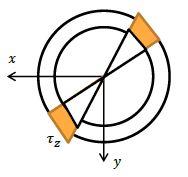
\includegraphics[width=0.3\linewidth]{figures/screenshot001}
	\label{fig:screenshot001}
\end{figure}
C'è poco spazio tra albero e primitiva, vuol dire che il piede del dente - a meno di correzioni - arriva molto vicino all'albero, andando a creare una zona di estrema concentrazione di tensioni. 

Realizzare poi una cava per linguetta porterebbe via troppo materiale resistente indebolendo troppo la ruota dentata. 

Questa scelta porta con sè il fatto che il materiale utilizzato per la ruota dev'essere lo stesso da utilizzare per l'albero, comportando un maggiore costo. \newline 

Se il rapporto tra diametro di primitiva e diametro dell'albero è tra $2,4\div4$ allora la ruota è un elemento a se stante calettato assialmente sull'albero. 
\begin{figure}[H]
	\centering
	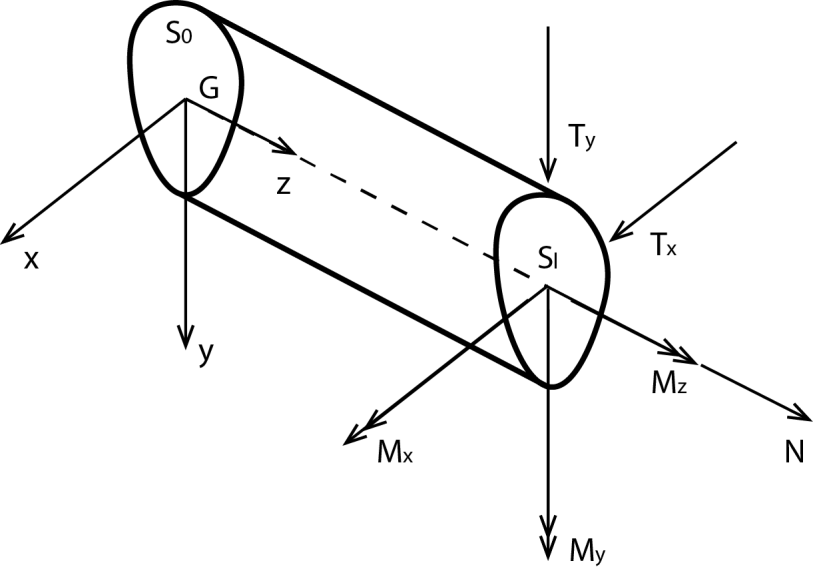
\includegraphics[width=0.3\linewidth]{figures/screenshot002}
	\label{fig:screenshot002}
\end{figure}
In proporziona all'albero la ruota dentata è piuttosto piccola, di conseguenza non c'è dimensione radiale tale da garantire una distinzione tra mozzo-corpo ruota-corona, per cui il corpo ruota scompare e la corona diventa un'unica parte col mozzo, la ruota si dice \textbf{piena}, la larghezza di fascia non supera mai una volta e mezza il diametro. \newline 

Se invece il rapporto supera il valore di 4, si potrà visualizzare ben distinta la parte centrale del corpo ruota dalla corona e dal mozzo. 

La dimensione assiale del mozzo non è mai superiore ad una volta e mezzo il diametro dell'albero.

Diviene più estesa per minimizzare le rotazioni della ruota rispetto all'albero, per renderla più solidale possibile rispetto all'albero. 
\begin{figure}[H]
	\centering
	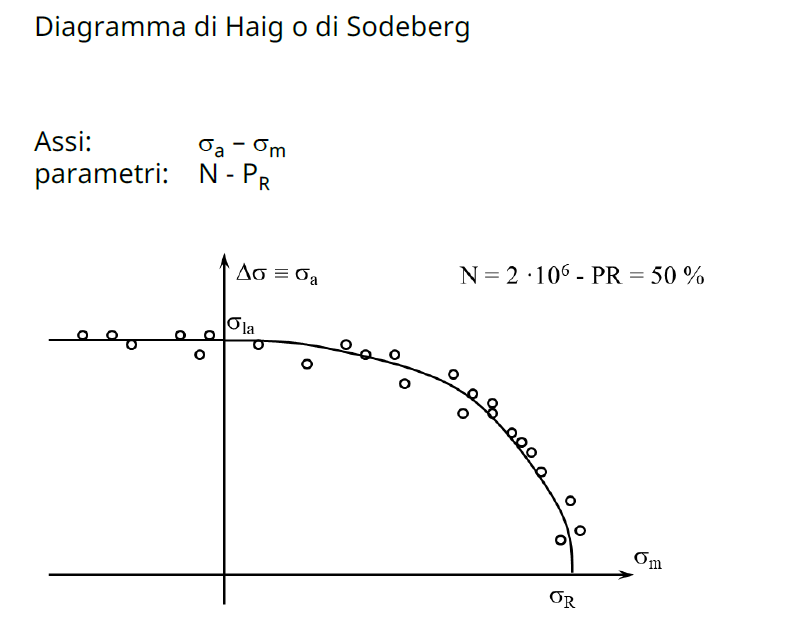
\includegraphics[width=0.3\linewidth]{figures/screenshot003}
	\label{fig:screenshot003}
\end{figure}
Mentre la sua larghezza è indipendente dalla larghezza del mozzo, sempre proporzionale al modulo della dentatura. \newline 

Se i diametri sono molto grandi, tramite realizzazione di fonderia si può optare per soluzione più tozze
\begin{figure}[H]
	\centering
	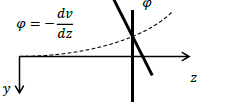
\includegraphics[width=0.3\linewidth]{figures/screenshot004}
	\label{fig:screenshot004}
\end{figure}

In alcuni casi poi ci si può permettere di alleggerire il corpo ruota, e quindi piuttosto che dimensionare un disco pieno (argomento di magistrale) si possono realizzare fori o razze. 

Il numero minimo di queste razze si attesta intorno a 
\[n = \left({1\over7}\div{1\over8}\right)\sqrt{D}\]
\begin{figure}[H]
	\centering
	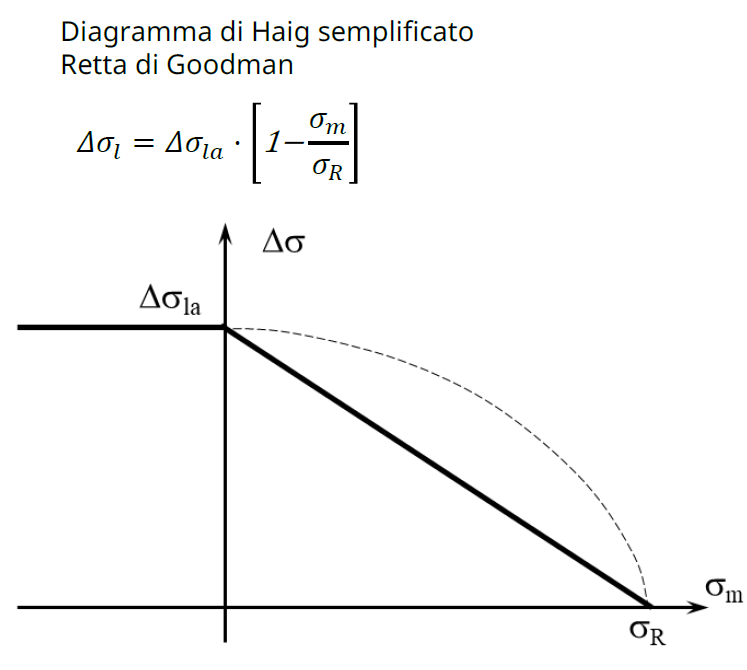
\includegraphics[width=0.3\linewidth]{figures/screenshot005}
	\label{fig:screenshot005}
\end{figure}
È sempre bene poi verificare il carico considerando le singole razze come degli elementi trave che con grande margine di sicurezza possono essere considerate incastrate al mozzo e libere sulla corona. 

La sezione delle razze può essere variabile 
\begin{figure}[H]
	\centering
	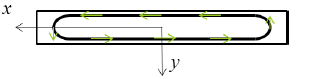
\includegraphics[width=0.3\linewidth]{figures/screenshot006}
	\label{fig:screenshot006}
\end{figure}

\begin{figure}[H]
	\centering
	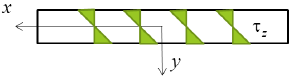
\includegraphics[width=0.3\linewidth]{figures/screenshot007}
	\label{fig:screenshot007}
\end{figure}

La scelta della sezione della razza sarà dettata dalla distribuzione dei carichi, nonché dalla tipologia dei denti. 

D'altronde una ruota a denti elicoidali ha anche una componente assiale, se questa è importante allora farà flettere la razza fuori dal piano della ruota, e quindi la sezione ad H rovesciato sarà la più indicata, perché ha un'inerzia maggiore in quella direzione, mentre una soluzione ad H dritta si può preferire per una ruota a denti dritti. 

	
\end{adjustwidth}
%\newpage
\section{Resistenza degli ingranaggi}
\begin{adjustwidth}{2in}{}
In realtà i carichi e la rigidezza sono tali da spostare l'attenzione, piuttosto che al mozzo o al corpo ruota, sulla dentatura. 

È molto più probabile che si porti a fine vita un  ingranaggio con un danneggiamento sul dente piuttosto che sul corpo ruota e sul mozzo. 

Questo perché sul dente accadono una certa quantità di fenomeni critici che possono portare alla rottura del dente a seconda della condizioni di funzionamento della ruota.\newline 

Le verifiche da apportare sono principalmente di 4 tipologie 
\begin{enumerate}
	\item \textbf{La resistenza a flessione del dente}: il carico transitante sul dente inflette il dente come se fosse una piccola trave incastrata sulla corona
	\begin{itemize}
		\item \textbf{Statica}
		\item \textbf{A fatica}
	\end{itemize}
	
	\item \textbf{Calcolo ad usura/pitting/vaiolatura}: basato sulla pressione Hertziana tra le parti, è un fenomeno legato alla forti pressioni  di contatto che localmente si generano sul profilo del dente. 
	
	\item \textbf{Verifica a grippaggio}: fenomeno che si instaura a causa dell'improvvisa sublimazione del lubrificante in particolari condizioni di temperatura portando a contatto diretto le superfici metalliche. 
	
	\item \textbf{Usura a marcia lenta}
\end{enumerate}

Le prime due verifiche sono le verifiche richieste dalla normative vigenti. \newline 

Storicamente l'attenzione si concentra sulla verifica a flessione. 

Il primo a teorizzare un modello valido dell'analisi tensionale sul dente di un ingranaggio è stato Lewis e stima con buona approssimazione la resistenza del dente, è la relazione di partenza con cui si effettua una stima del modulo da assegnare alla ruota dentata. 

Tuttavia è un modello semplificato perché  il problema di resistenza del dente è estremamente complesso già a partire dagli input da inserire nel modello: l'effettivo carico sul dente, se non viene misurato sperimentalmente, è estremamente complesso da ricavare analiticamente. \newline

Il carico per buona approssimazione è costante durante tutto l'ingranamento, per direzione, verso e intensità: dicendo questo si sta già teorizzando un ingranaggio con un solo dente in presa, e nella realtà ciò non è auspicabile. 

Nella realtà teorico-pratica il contatto avviene tra più denti: si prende in utilizzo la metà del carico sgravando il dente che sta uscendo dall'ingranamento in virtù del fatto che il dente può essere modellizzato come un sistema iperstatico con una ripartizione del carico dipendente dalle rigidezze dei denti, questi uguali tra loro.

Tuttavia le rigidezze del sistema sono diverse in accesso e in recesso, la ripartizione del carico non è perfettamente ed equamente ripartita. \newline

L'intensità è costante in direzione solo nel sistema di riferimento globale, rispetto al sistema di riferimento locale, orientato secondo l'asse del dente, è invece variabile. \newline 

Inoltre a seguito delle flessioni dell'albero e della deformabilità della ruota, le superfici di contatto cambiano durante l'ingranamento. \newline 

Un effettivo carico sul dente si può calcolare  soltanto sperimentalmente con complessi sistemi di misura.  
\end{adjustwidth}
%\newpage
\section{Modello di Lewis per la flessione}
\begin{adjustwidth}{2in}{}
Il modello di Lewis è cautelativo, conservativo. 
\begin{figure}[H]
	\centering
	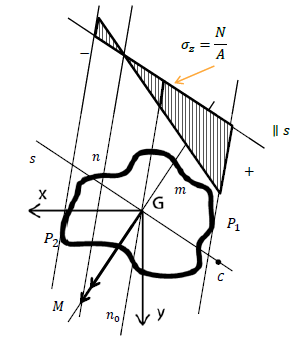
\includegraphics[width=0.5\linewidth]{figures/screenshot008}
	\caption{Ripartizione del carico durante l'ingranamento.}
	\label{fig:screenshot008}
\end{figure}
$E_1, E_2$ sono i punti estremali del contatto. 

Secondo l'approssimazione di Lewis  in accesso e in recesso avverrà un contatto doppio mentre sarà singolo al centro. \newline 

Lewis si è messo in condizioni conservative applicando il carico sulla punta del dente, ovvero dove finisce l'evolvente del dente. 

Il carico si applica sulla testa del dente come se fosse l'unico dente in presa ed inclinato secondo un angolo $\beta$ rispetto all'asse ortogonale del dente. \newline 

Le approssimazioni cautelative sono parecchie 
\begin{enumerate}
	\item Si prende tutto il carico applicato sul dente, come se ce ne fosse solo uno in presa. 
	
	Il dente si comporta così solo quando si trova in \textit{contatto singolo}. 
	
	\item Si prende come punto d'applicazione quello con maggiore braccio. 
	
	\item Sulla testa del dente l'inclinazione della forza rispetto all'asse del dente è molto più grande: la forza  scambiata, che segue sempre l'angolo di pressione nel sistema di riferimento globale, avrà un angolo completamente diverso rispetto all'asse: $\beta\ne\theta$.
	
	L'approssimazione di Lewis dice invece di considerare sulla testa del dente un angolo di applicazione pari all'angolo di pressione $\beta=\theta$. 
	
	\item Considera il dente come una trave incastrata alla De Saint Venant, sapendo bene che questa è modellizzabile come una trave molto tozza, non studiabile con De Saint Venant. 
\end{enumerate}

\begin{figure}[H]
	\centering
	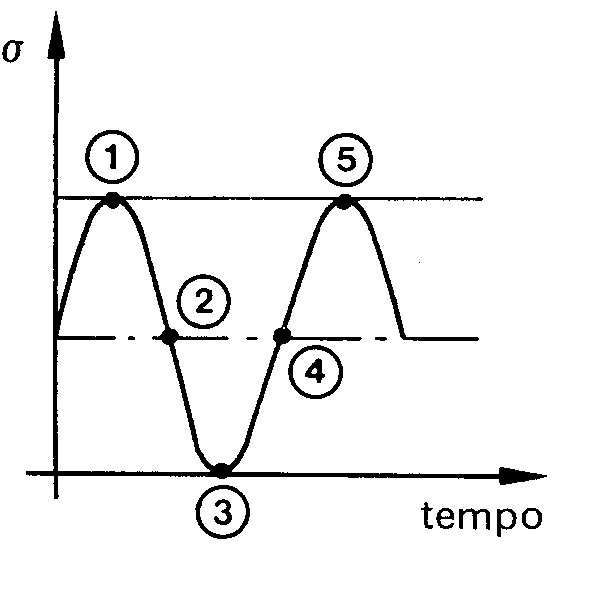
\includegraphics[width=0.\linewidth]{figures/screenshot009}
	\label{fig:screenshot009}
\end{figure}
\newpage
Questa trave sarà sollecitata dal carico 
\[\dfrac{Q}{\cos\theta}\]
Inclinato di un angolo $\beta=\theta$.

Operando un trasferimento del carico lungo la sua retta d'azione fino ad incontrare l'asse del dente, questo si troverà in posizione M
\begin{figure}[H]
	\centering
	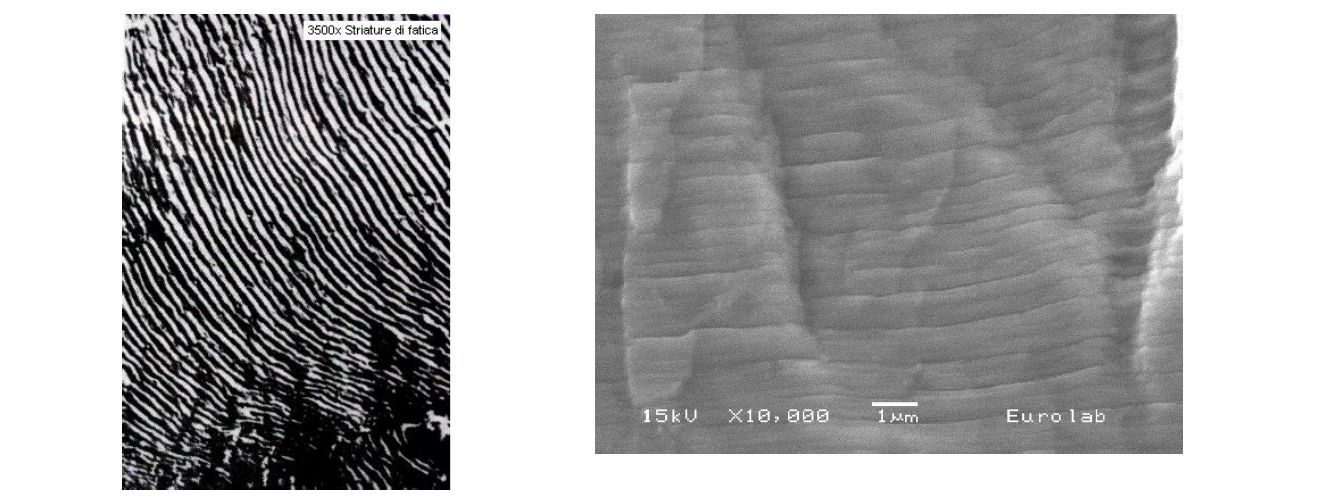
\includegraphics[width=0.\linewidth]{figures/screenshot010}
	\label{fig:screenshot010}
\end{figure}
La trave diviene così caricata da una sollecitazione di taglio $T$ e da sforzo normale pari ad $N$
\[T = Q\dfrac{\cos\beta}{\cos\theta} \qquad N = T\tan\beta\]
La sollecitazione ad un determinato spessore a quota $z=B$ sarà data da una componente di flessione 
\[\sigma_f = \dfrac{6Tz}{s^2b}\]
E da una componente di compressione 
\[\sigma_c = -\dfrac{T}{sb}\tan\beta\]
E da una sollecitazione di taglio, che per sezione rettangolare 
\[\tau_{medio} = \dfrac{T}{sb} \qquad \tau_{max} = 1,5\tau_{medio}\]

Siccome ci si è messi in forte conservatività sui carichi, l'approccio di Lewis ipotizza che la sollecitazione di taglio e quella di compressione non comportino criticità 
\begin{itemize}
	\item La sollecitazione di compressione non apre cricche di fatica
	\item Il taglio è massimo dov'è nulla la sollecitazione di pressione
\end{itemize}
Valutando unicamente solo la componente di pressione. \newline 

Per cui la tensione di flessione alla Lewis diviene 
\[\sigma_L = \dfrac{6Qz}{s^2b}\]
Questo è un andamento della tensione di flessione in funzione della quota $z$, solo che il dente non è una trave alla DSV a sezione costante. \newline 

Si individueranno così le situazioni critiche laddove ci siano spessori minori in punti di incastro. 

\begin{en}
	Una trave a sezione rettangolare sarebbe a iso-resistenza (presentando la stessa tensione lungo tutto il bordo della sezione) se avesse una delle due dimensioni della sezione rettangolare (e.g. base costante e altezza variabile), con una legge di variazione del lato variabile di forma parabolica. 
\end{en}

Per cui se la trave a sezione rettangolare considerata anziché avere una sezione constante  avesse l'altezza del rettangolo variabile con legge parabolica, allora tutti i punti del fianco della trave avrebbero tutti la stessa tensione di flessione. 

\newpage

Questa legge parabolica si può scrivere come 
\[y = k\sqrt{z}\]
Con $k$ coefficiente di amplificazione della parabola in funzione del livello di tensione raggiunto o raggiungibile.

La massima tensione si può così avere per la parabola più grande inscritta nel profilo del dente. 

Il punto di tangenza di questa parabola col profilo del dente sarà il punto più sollecitato del dente, in questo caso il punto $H$. 

Sostituendo nei i valori di tensioni trovati le dimensioni tipiche della sezione più sollecitata (apice '), si giunge a 
\[\sigma_L = \dfrac{Q}{\dfrac{1}{6}\dfrac{s'}{z'}\dfrac{s'}{m}mb} = \dfrac{Q}{ymb} \qquad y = \dfrac{s'^2}{6z'm}\]
Individuando così il termine $y$ che determina la sezione più sollecitata. \newline 

Invertendo tale relazione si trova il carico ammissibile 
\[Q_{amm} = \sigma_{amm}ymb\]
Cioè imponendo che la tensione di flessione  sia pari all'ammissibile di resistenza del dente, si trova quale sia il carico ammissibile transitante per un singolo dente. \newline 

La $y$ così individuata dipende dell'angolo di pressione, dall'inviluppo di realizzazione, dal numero di denti... Dev'essere ricavata geometricamente. 

Per ricavare una relazione di progetto si parte dal fatto che $Q$ è proporzionale al momento torcente transitante, 
\[M = QR = Q\dfrac{zm}{2} \Rightarrow Q = \dfrac{2M}{zm} = ymb\sigma_{amm}\]
Introducendo il fatto che la larghezza di fascia è pari a 
\[b = \lambda m\]
Dove per i denti dritti $\lambda = 8\div12$ e per i denti elicoidali $\lambda=10\div30$.

Allora si può scrivere 
\[Q = ym^2\lambda\sigma_{amm}\]
Moltiplicando per la stessa quantità 
\[mQ = mym^2\lambda\sigma_{amm}\]
Sostituendo $Q$ si ottiene
\[\dfrac{2M}{z} = ym^3\lambda\sigma_{amm}\]
Esplicitando il modulo
\[m = \underbrace{\sqrt[3]{\dfrac{2}{zy}}}_{k}\cdot\sqrt[3]{\dfrac{M}{\lambda\sigma_{amm}}}\]
Infine 
\[m =k\sqrt[3]{\dfrac{M}{\lambda\sigma_{amm}}}\]
La $\sigma_{amm}$ è quella propria del materiale considerando tuttavia un fattore di sicurezza per a 3 o a 5. \newline 

L'approccio di Lewis è - come detto - semplificato, quindi da solo non può essere la verifica di resistenza a flessione del dente, però può essere una relazione di primo dimensionamento del dente. 

Per cui proprio come si faceva per l'albero in cui il primo diametro si ricavava a partire da una relazione statica di flessione con un'importante fattore di sicurezza sull'ammissibile, questa relazione verrà utilizzata per una prima scelta del modulo del dente utilizzando un opportuno fattore di sicurezza sull'ammissibile statica del materiale della ruota. 

Per la ruota a denti dritti, si individua così un primo modulo della dentiera, per le ruote a denti elicoidali invece quello non è affatto il modulo della dentiera - quello sul piano normale - ma quello sul piano frontale perché la forza utile è lì che giace! 	

Questa relazione per le ruote dentate elicoidali tira fuori il modulo frontale di funzionamento, dal quale è possibile ricostruire il modulo della dentiera attraverso equazioni già note. \newline 

\begin{figure}[H]
	\centering
	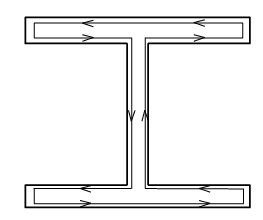
\includegraphics[width=1\linewidth]{figures/screenshot011}
	\caption{$k$ della relazione di Lewis}
	\label{fig:screenshot011}
\end{figure}

Se i calcoli a resistenza non vengono fatti adeguatamente, queste saranno le conseguenze.
\begin{figure}[H]
	\parbox{0.60\textwidth}{\centering
	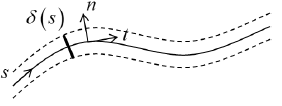
\includegraphics[width=1\linewidth]{figures/screenshot012}
	\label{fig:screenshot012}}
\hfill
	\parbox{0.45\textwidth}{\centering
	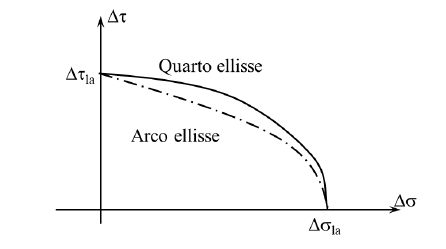
\includegraphics[width=1\linewidth]{figures/screenshot013}
	\label{fig:screenshot013}}
\end{figure}

La cricca di pressione a fatica parte proprio dalla base del dente. 

Tuttavia nell'approccio di Lewis questa variazione di forma non c'è: il calcolo prevede una trave con spessore variabile senza valutare concentrazioni  di tensioni teoriche dovute alle variazioni di forma ed è una grande pecca di questo modello. 
\end{adjustwidth}
%\newpage
\section{Resistenza a pitting}
\begin{adjustwidth}{2in}{}
	Un altro fenomeno di criticità è quello della vaiolatura (pitting). 
	
	In questo caso non è una rottura del dente  a portare il malfunzionamento della ruota dentata ma un danneggiamento della superficie del dente. 
	
	Qual è la conseguenza? Se si danneggia la superficie del dente si perdono le condizioni di ingranamento corretto secondo l'evolvente, ma al tempo stesso una grande quantità di materiale viene espulsa e finisce nel bagno  d'olio interponendosi successivamente tra i denti durante l'ingranamento portando al bloccaggio dell'ingranaggio. 
	\begin{figure}[H]
		\parbox{0.45\textwidth}{\centering
		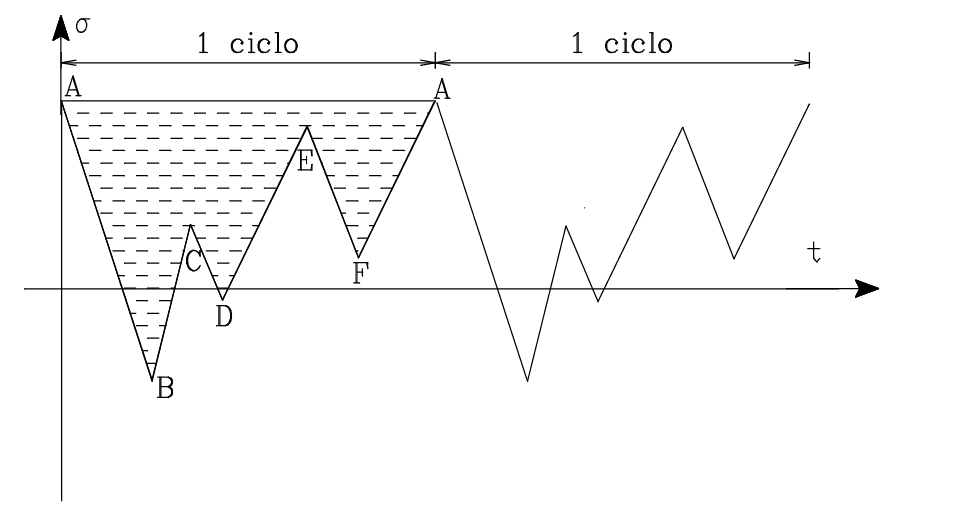
\includegraphics[width=1\linewidth]{figures/screenshot014}
		\label{fig:screenshot014}}
	\hfill
	\parbox{0.45\textwidth}{\centering\centering
		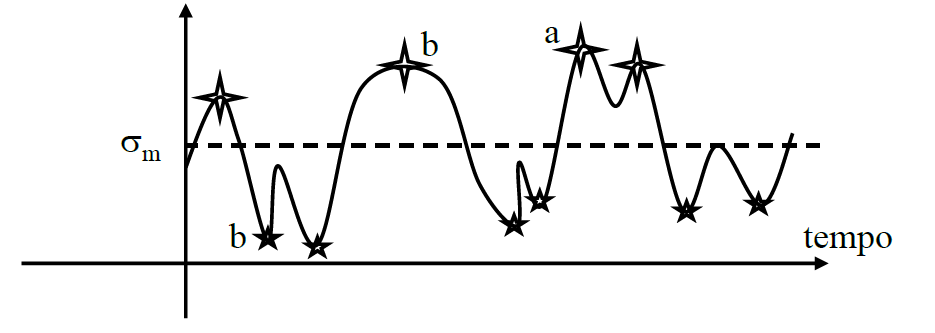
\includegraphics[width=1\linewidth]{figures/screenshot015}
		\label{fig:screenshot015}}
	\end{figure}
	Questa superficie così butterata e ruvida, incoerente, viene generata  dall'eccessivo carico di pressione di contatto sulle superfici. 
	
	Questa pressione di contatto hertziana tra le superfici genera uno stato tensionale sotto-pelle che porta ad un distaccamento del materiale a causa proprio del cedimento locale del materiale
	\begin{figure}[H]
		\centering
		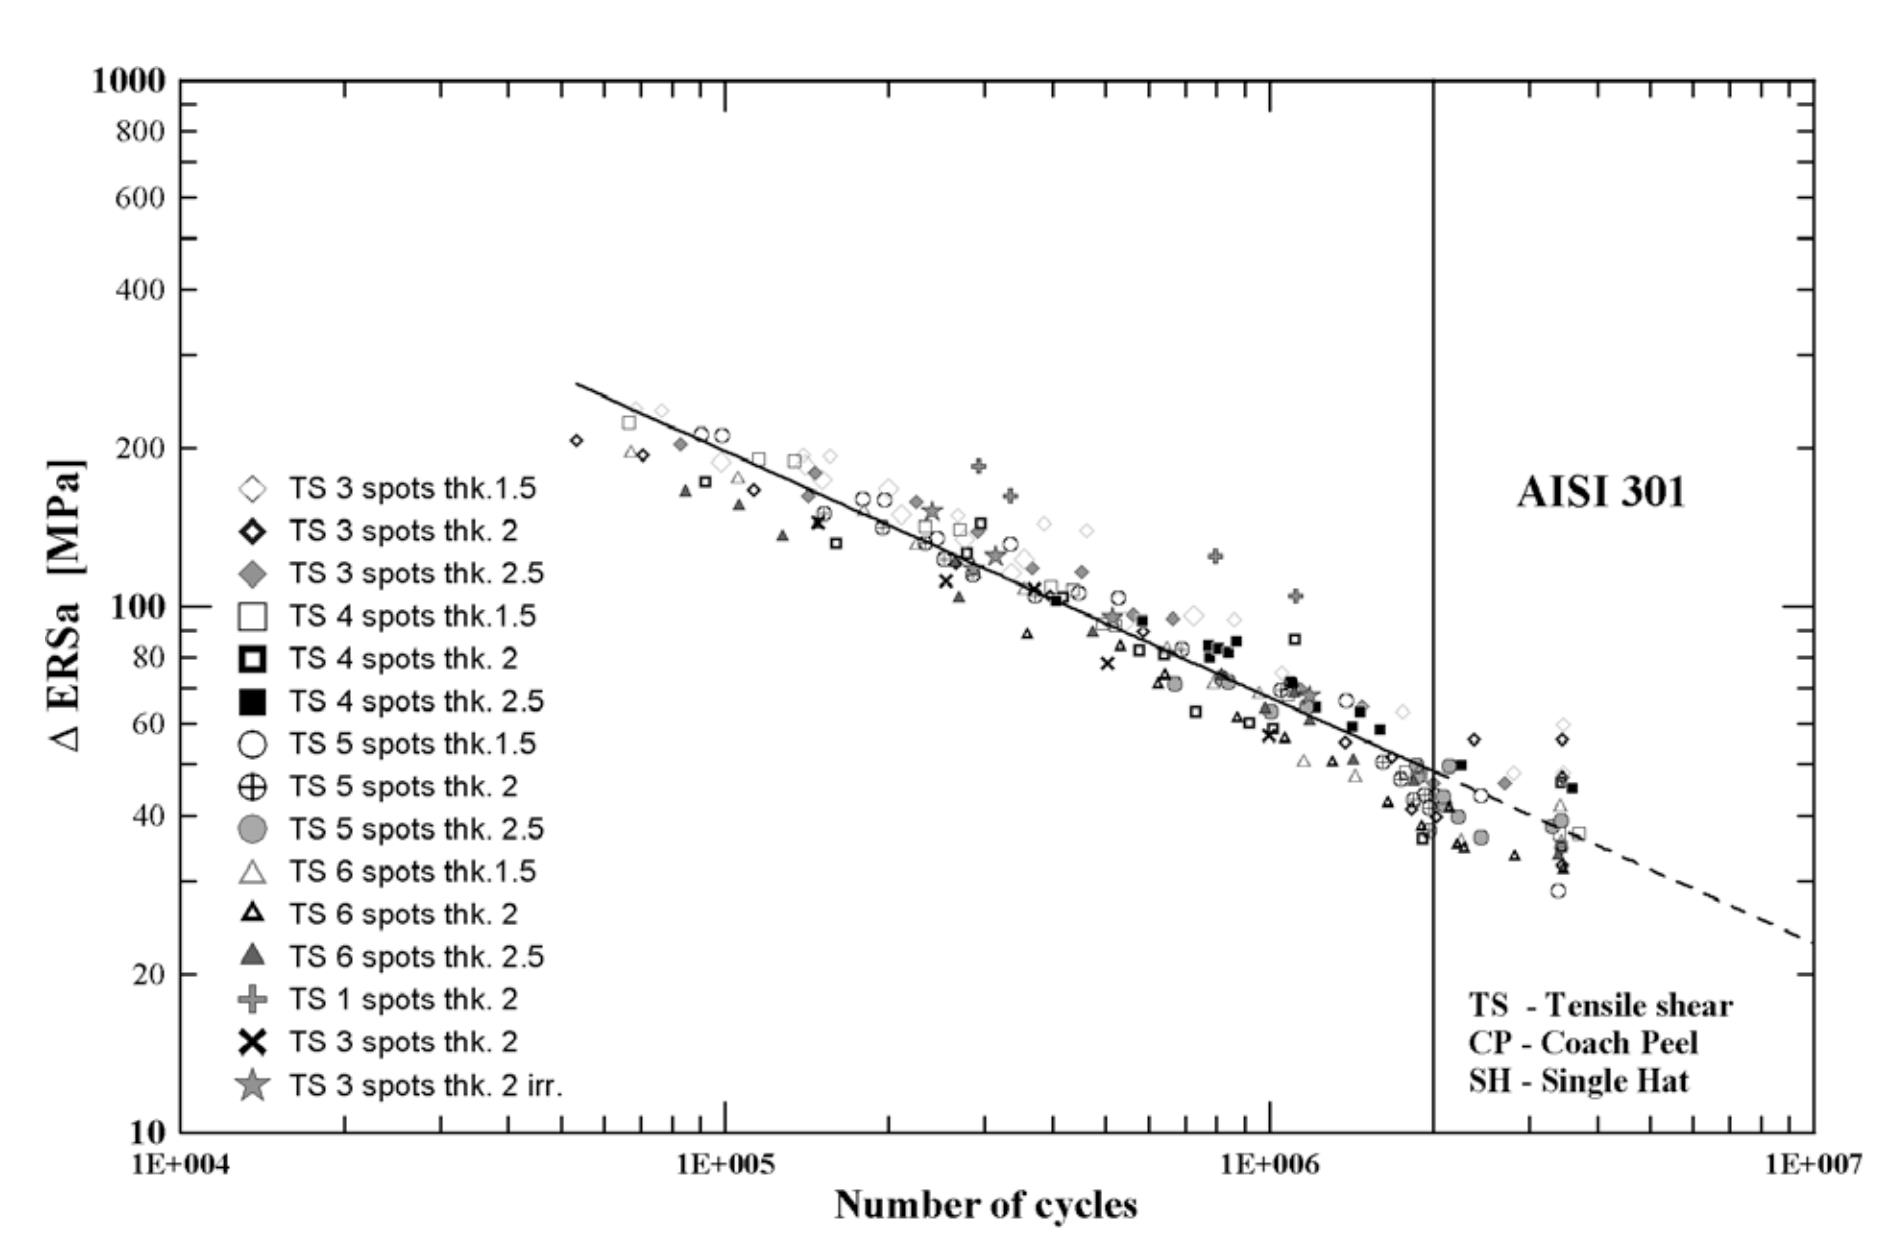
\includegraphics[width=0.5\linewidth]{figures/screenshot016}
		\label{fig:screenshot016}
	\end{figure}
	Può essere può o meno estesa ma comunque porta al distaccamento dal fianco del dente di una grande quantità di materiale. \newline 
	
	Il fenomeno del pitting  si presenta molto più frequentemente sugli acciai da bonifica. 
	
	Confrontando la resistenza dei materiali ai vari fenomeni citati finora. 
	\begin{figure}[H]
		\centering
		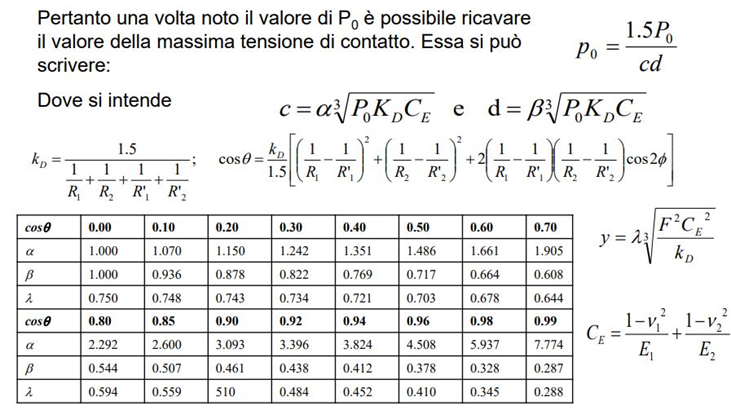
\includegraphics[width=1\linewidth]{figures/screenshot017}
		\label{fig:screenshot017}
	\end{figure}
	Finché non c'è stato un sufficiente sviluppo dei materiali, la vaiolatura era la maggior causa di rottura delle ruote dentate. 
	
	Il passaggio ad acciai da cementazione (acciai legati a basso tenore di carbonio) ha innalzato il limite molto più in alto, permettendo di concentrare gli sforzi sulla resistenza a flessione del dente.  
\newpage	
	Come quantificare il pitting?
	
	La corretta valutazione  dello stato tensionale sul dente è legata alla valutazione della pressione hertziana, questa è un carico per unità di superficie, dettato dalle caratteristiche del materiale, ma anche dalle forme delle superficie in contatto, e quindi dai raggi di curvatura delle due superfici che si toccano. 
	\begin{figure}[H]
		\centering
		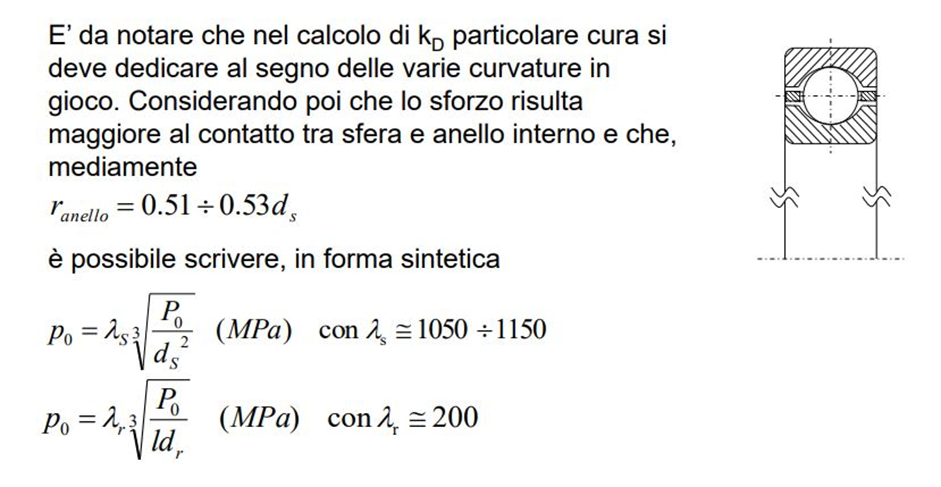
\includegraphics[width=0.5\linewidth]{figures/screenshot018}
		\caption{}
		\label{fig:screenshot018}
	\end{figure}	
	La tensione hertziana teorica si scrive come 
	\[\sigma_H = \sqrt{\dfrac{Q}{b\cos\theta} \cdot \dfrac{\rho}{\pi\Delta}}\] 
	In cui 
	\begin{itemize}
		\item $\dfrac{Q}{b\cos\theta}$ è il carico lineare per unità di larghezza di fascia. 
		\item $\rho$ è il termine geometrico che tiene conto delle curvature principali delle superfici 
		\[\rho = \dfrac{1}{MT} + \dfrac{1}{MT'}\]
		\item $\Delta$ raccoglie le proprietà elastiche dei materiali 
		\[\Delta = \dfrac{1-\nu_1^2}{E_1} + \dfrac{1-\nu_2^2}{E_2}\]
	\end{itemize}
	Sostituendo il Poisson tipico degli acciai e considerando lo stesso materiale per ruota e per pignone, si ottiene 
	\[\sigma_H^{\max} = 0.418\sqrt{\dfrac{QE\rho}{b\cos\theta}}\]
	Per definire $\rho$ basta passare dalla geometria
	\[\begin{dcases}
		MT = R\sin\theta + \delta \\
		MT' = R'\sin\theta - \delta
	\end{dcases}\]
	Per cui
	\[\rho = \dfrac{(R+R')\sin\theta}{(R\sin\theta+\delta)(R'\sin\theta+\delta)}\]
	Con $\delta$ ascissa curvilinea che misurava la distanza del punto di contatto da centro di istantanea rotazione. \newline 
	
	La pressione hertziana varia così lungo il segmento dei contatti, con un andamento simile. 
	\begin{figure}[H]
		\centering
		
\includegraphics[width=0.5\linewidth]{figures/screenshot019}
		\label{fig:screenshot019}
	\end{figure}
	Riportando il grafico delle tensioni hertziane massime si individua un valore infinito in $T, T'$ per poi decrescere fino ad un minimo osservato ne punto $H$. \newline 
	
	\textbf{Osservazioni}
	\begin{enumerate}
		\item È finita laddove finisce l'evolvente, giammai avvicinarsi alla circonferenza fondamentale. 
		\item Il punto $H$ NON è il centro di istantanea rotazione. 
		
		Mentre gli strisciamenti specifici sono nulli nel centro di istantanea rotazione, la pressione non è minima  nel centro di istantanea rotazione. 
		
		Un breve studio di funzione identifica infatti un valore minimo nel punto
		\[\delta_{\min} = {1\over2}(R'-R)\sin\theta\]
		Ovvero a metà del segmento teorico dei contatti. 
		
		Questo valore sostituito all'interno della formulazione di $\rho$ porta a 
		\[\rho_{\min} = {4\over L}\dfrac{1}{1-\left(\dfrac{\delta-\delta_{\min}}{L}\right)^2}\]
		Con $L=(R+R')\sin\theta$. 
		
		Questo valore è a sua volte sostituibile nella funzione $\sigma^{\max}_H$ ricavando quanto vale la minima pressione hertziana in quel punto. 
	\end{enumerate}
	\vspace{0.5cm}
	La tensione hertziana è massima laddove sia massimo $\rho$ e quindi in $T, T'$, allora se si limita il segmento dei contatti al segmento effettivo  determinato dalle troncature esterne di ruota e pignone, il valore di $\sigma$ sarà si elevato ma non più infinito. 
	
	In realtà questa tensione (figura \ref{fig:screenshot018}) si manifesterebbe quando durante l'ingranamento la coppia dei denti in  presa fosse sempre e solo una, ma quando inizia il contatto è almeno una coppia, e allora considerando la distribuzione di forze teorica (figura \ref{fig:screenshot008}), la funzione hertziana si riduce notevolmente in ingresso e in uscita. 
	\begin{figure}[H]
		\centering
		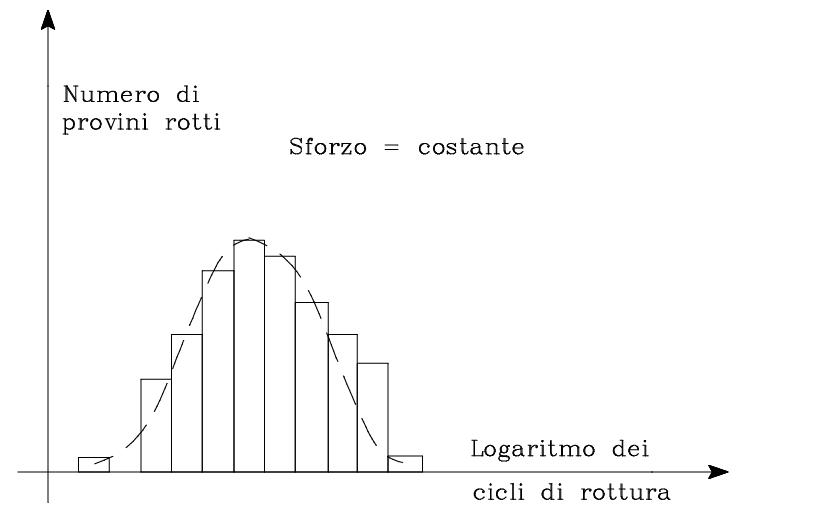
\includegraphics[width=0.3\linewidth]{figures/screenshot020}
		\label{fig:screenshot020}
	\end{figure}
	Ne consegue che non sarà l'inizio del contatto il punto con maggior pressione hertziana, ma sarà il punto B in figura caratterizzato da $\rho_{0}$. \newline 
	
	Dal punto di vista pratico sussistono due approssimazioni, il fatto che la forza in ingresso non sia la metà (sperimentalmente è di più) e per il fatto che - sperimentalmente - il fenomeno del pitting non si manifesta in B ma esattamente nel centro di istantanea rotazione. \newline 
	
	La verifica a pitting si fa perciò in C, a $\delta=0$. 
	
	Questo perché le ipotesi di Hertz non sono sempre garantite:
	\begin{enumerate}
		\item Corpi perfettamente elastici: ipotesi reale
		\item Superfici asciutte: ipotesi negata dalla lubrificazione
	\end{enumerate}
	Correggendo le relazioni hertziane considerando anche la lubrificazione la lubrificazione che ne risulta è questa 
	\[\sigma_H^{\max} = 0.59\sqrt{\dfrac{Q}{b}\dfrac{E}{\sin^2\theta}\dfrac{1+\tau}{R}}\]
	Correggendola attraverso la modifica del fattore numerico e l'inserimento del rapporto di trasmissione. 
	
	Questa relazione è utile per ricavare a ritroso un'equazione di progetto simile a quella di Lewis
	\[Q = cmb \]
	Dove
	\[c = \dfrac{\sin2\theta}{0,696}\dfrac{\sigma_{max}^2}{e}\dfrac{z}{1+\tau}\]
	Esplicitando la tensione ammissibile si può così trovare il carimc massimo per pitting 
	\begin{figure}[H]
		\centering
		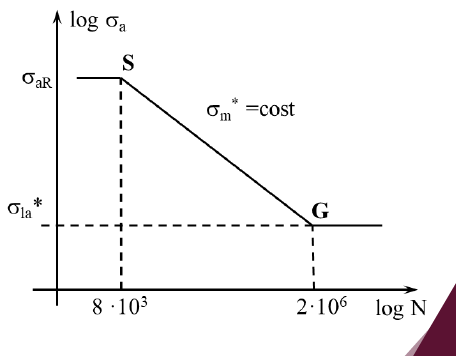
\includegraphics[width=1\linewidth]{figures/screenshot021}
		\caption{Tensioni massime}
		\label{fig:screenshot021}
	\end{figure}
	Evidenziando valori totalmente diversi da quelli visti per la resistenza a flessione. 
	
	Notare come i valori massimi dipendano dall'accoppiamento dei due materiali. \newline 
	
	La scelta della tensione ammissibile è legata ad evidenze sperimentali o alla durezza Brinell o alle caratteristiche elastiche del materiale, secondo normativa. 
	
	Attualmente le Normative ISO prevedono una verifica a flessione e a pitting. 
	
	Tali normative, pur basandosi sul ragionamento di Lewis, introducono alcune modifiche proposte da Neimann e alcuni coefficienti che prendono in considerazione ulteriori fattori che concorrono alla resistenza. 
\end{adjustwidth}
\newpage
\section{Effetto d'intaglio alla radice del dente}
\begin{adjustwidth}{2in}{}	
	Primo fra tutti i fattori di correzione, viene introdotto quello di concentrazione di tensione alla base del dente  dovuto alle variazioni di forma. 
	
	Il valore di tensione di flessione sarà un valore nominale al quale andrà aggiunto il $K_t$. 
	
	Ragionando  su fenomeni di fatica, tale $K_t$ ha senso di esistere anche su materiali duttili come  gli acciai di comune impiego per le ruote dentate. \newline 
	
	Questo fattore di concentrazione di tensione viene introdotto attraverso modelli articolati in funzione del raggio di piede. 
	\begin{figure}[H]
		\centering
		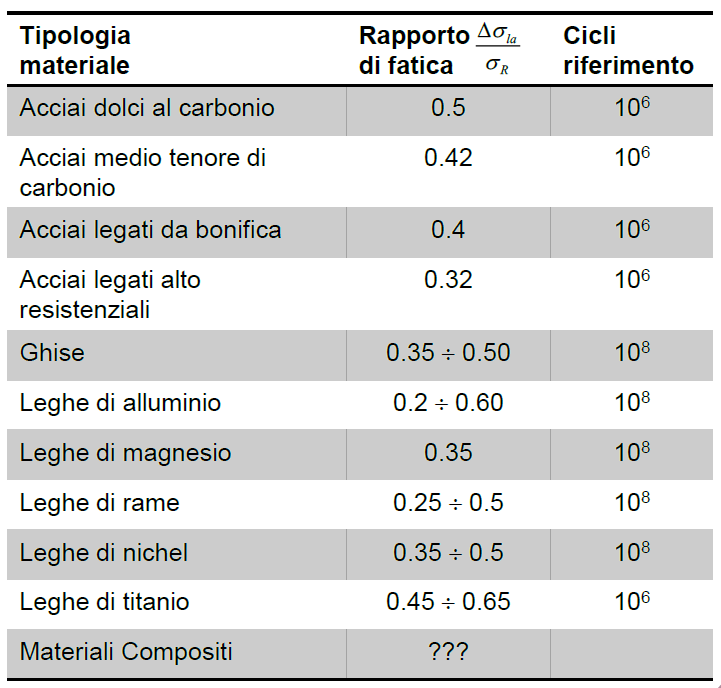
\includegraphics[width=0.5\linewidth]{figures/screenshot022}
		\label{fig:screenshot022}
	\end{figure}
	Ed in funzione del rapporto tra altezza e spessore del dente
	\begin{figure}[H]
		\centering
		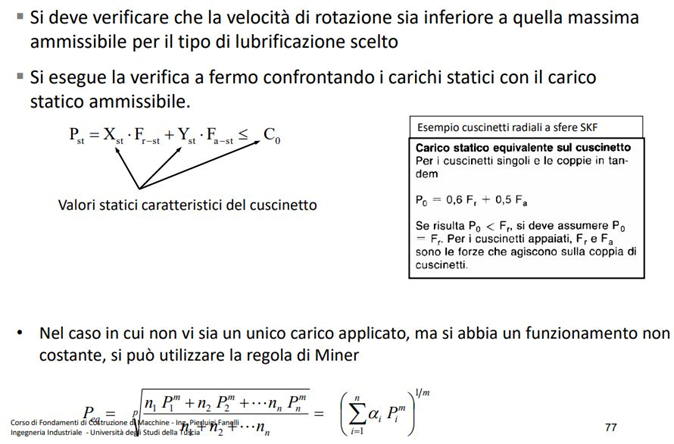
\includegraphics[width=0.5\linewidth]{figures/screenshot023}
		\label{fig:screenshot023}
	\end{figure}
	Questi studi vengono raccolti da Neimann che li avvicina alla realtà allontanandosi dalle considerazioni conservative di Lewis. 
\end{adjustwidth}
\newpage
\section{Modello di Neimann per la flessione}
\begin{adjustwidth}{2in}{}	
	La prima modifica risiede nell'individuazione della sezione critica, che non avviene più mediante una parabola inscritta all'interno del profilo del dente, ma mediante l'inscrizione nel profilo del dente di un triangolo equilatero, che ne punto di tangenza del profilo individua ul punto di massima tensione. 
	
	la seconda modifica che introduce riguarda l'applicazione del carico, questo infatti non verrà più posto agente sulla testa del dente, bensì nell'effettiva posizione ultima in cui si ha il contatto singolo. 
	
	Considerando l'effettiva inclinazione dell'applicazione della forza. 
	\begin{figure}[H]
		\centering
		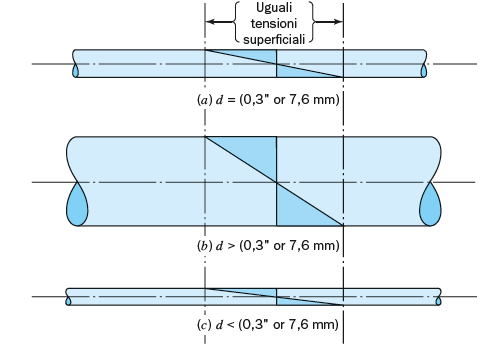
\includegraphics[width=0.3\linewidth]{figures/screenshot024}
		\label{fig:screenshot024}
	\end{figure}
	Questo risulta così un modello più realistico e meno conservativo.\newline 
	
	Rispetto a Lewis, secondo Neimann sarà 
	\[\sigma_N = \dfrac{6h_1Q\cos\beta}{bs_F^2\cos\theta} = \dfrac{6\left(\dfrac{h_1}{m}\right)^2mQ\cos\beta}{b\left(\dfrac{s_F}{m}\right)^2m^2\cos\theta} = \dfrac{Q}{mb}Y_F\] 
	Con $Y_F$ fattore di forma. 
	
	Questa sarà la tensione nominale e avrà un andamento a farfalla perfettamente centrato alla base del dente. \newline 
	
	Il valore effettivo di tensione Neimann lo ricava correggendo la tensione nominale attraverso una $Y_S$, questa funzione di 
	\[Y_S=(1,2+0,13L)q_s^{{1\over1.21 + {2.3\over L}}}\]
	Dove $L=\dfrac{s_F}{h_1}, q_s = \dfrac{s_F}{2\rho_F}$ 
	
	Questo approccio implica la conoscenza  del punto di contatto reciproco tra i denti, l'altezza $h_1$ dipende da tutto l'ingranamento: l'ultimo punto di contatto dipende dal cinematismo dell'ingranaggio e quindi dipende dalla ruota coniugata. \newline
	
	Di conseguenza si preferisce avere una relazione che dipenda esclusivamente dalla ruota in esame, se ci si riporta ad applicare la forza sulla testa del dente, questa sarà sempre la stessa indipendentemente dall'accoppiamento coniugato, e quindi correggere Neimann utilizzando l'altezza del dente $h_2$ al posto di $h_1$. 
	
	Naturalmente tale scelta porta con sè un momento flettente maggiore, aggravando il carico ma tornando ad avere un'effettiva stima della resistenza indipendente dal montaggio effettivo. 
	
	Considerando il carico in testa si aggiungerà un pedice $t$ alle ban note grandezze fin'ora introdotte. 
	\[Y_{Ft} \quad Y_{St} \quad \sigma_{Ft}\]
	
	I tue approcci possono essere legati attraverso un fattore di correzione $Y_\varepsilon$ che dipende dal fattore di ricoprimento (SOLO RELATIVO ALL'EVOLVENTE). 
	\[Y_\varepsilon = 0.25 + \dfrac{0.75}{\varepsilon}\]
	E quindi
	\[\sigma_{F0} = \dfrac{Q}{bm}Y_FY_S = \dfrac{Q}{bm}Y_{Ft}Y_{St}Y_\varepsilon\]	
	\begin{figure}[H]
		\centering
		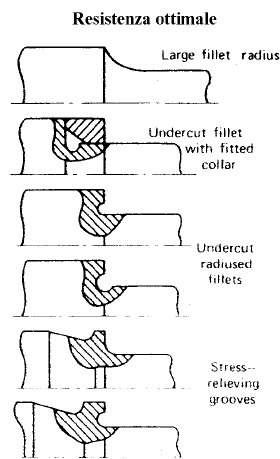
\includegraphics[width=0.7\linewidth]{figures/screenshot025}
		\caption{Fattore di forma}
		\label{fig:screenshot025}
	\end{figure}
In alternativa ai grafici, la normativa fornisce anche delle formule. 	
	 \begin{figure}[H]
	 	\centering
	 	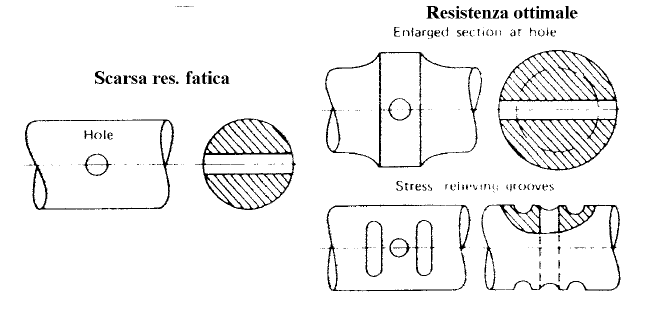
\includegraphics[width=0.7\linewidth]{figures/screenshot026}
	 	\label{fig:screenshot026}
	 \end{figure}
	 \begin{figure}[H]
	 	\centering
	 	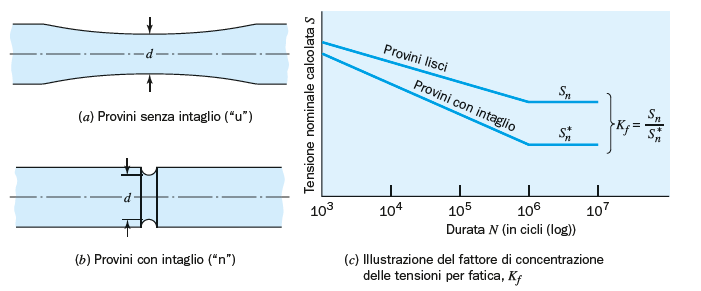
\includegraphics[width=0.7\linewidth]{figures/screenshot027}
	 	\label{fig:screenshot027}
	 \end{figure}
	 \begin{figure}[H]
	 	\centering
	 	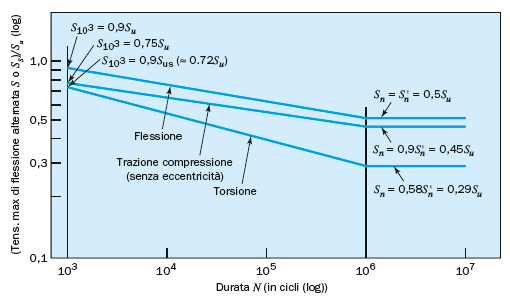
\includegraphics[width=0.7\linewidth]{figures/screenshot028}
	 	\label{fig:screenshot028}
	 \end{figure}	 
\end{adjustwidth}
\newpage
\section{Verifica a flessione secondo UNI 8862 ISO C}
\begin{adjustwidth}{2in}{}
	Il picco di tensione è pari alla tensione di Neimann in testa al dente moltiplicato per un fattore che tiene conto  dell'eventuale elicoidalità della dentatura. 
	\[\sigma_{F0} = \dfrac{Q}{bm}Y_{Ft}Y_{St}Y_\varepsilon Y_\beta\]
	Tale normativa introduce inoltre una serie di fattori maggiorativi dello stato tensionale, dovuto a tutti quegli effetti non presi in considerazione da Neimann 
	\[\sigma_{F} = \sigma_{F0}K_AK_VK_{F\beta}K_{F\alpha}\]
	\begin{figure}[H]
		\centering
		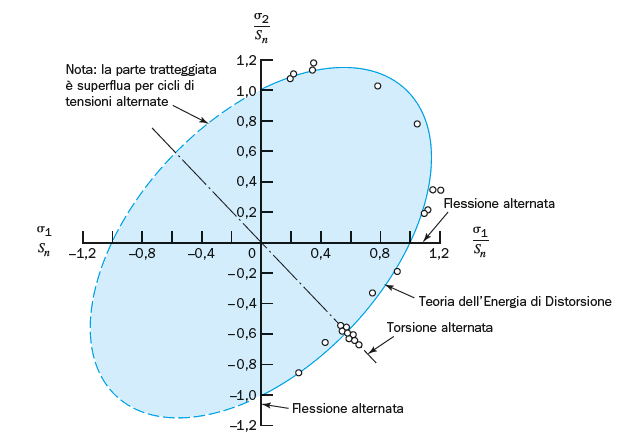
\includegraphics[width=1\linewidth]{figures/screenshot029}
		\label{fig:screenshot029}
	\end{figure}
	La valutazione dei coefficiente $K_i$ avviene secondo un procedimento indicato nella normativa. \newline 
	
	Tale valore di sforzo sul dente dev'essere confrontato con la tensione ammissibile.
	\[\sigma_{FP}=\dfrac{\sigma_{Flim}}{F_{Flim}}Y_{ST}Y_{NT}Y_{\delta relT}Y_{Rrel T}Y_X\]
	\begin{figure}[H]
		\centering
		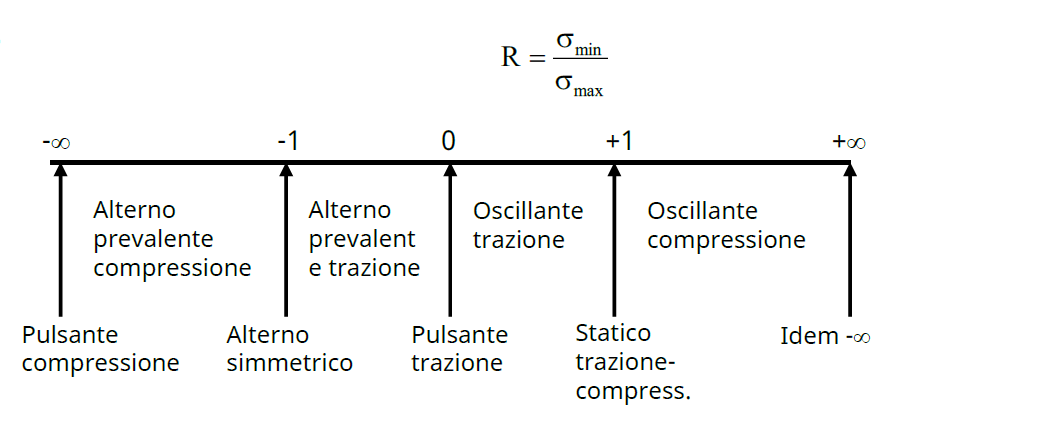
\includegraphics[width=1\linewidth]{figures/screenshot030}
		\label{fig:screenshot030}
	\end{figure}	
	Deve ovviamente risultare che la tensione di picco della flessione dev'essere minore di quella ammissibile
	\[\sigma_{F}\leq\sigma_{FP}\]
	
	Tale verifica dovrebbe essere effettuata anche in condizioni statiche, tuttavia la normativa afferma che è sufficiente considerare un numero di cicli inferiori a $10^3$, al limite della fatica oligociclica. 
\end{adjustwidth}
\newpage
\section{Verifica a pitting secondo UNI 8862 ISO C}
\begin{adjustwidth}{2in}{}	
	L'approccio per la verifica a pitting è similare a quello  visto per la flessione, si prende la teoria hertziana e si corregge con una serie di fattori amplificati dalle condizioni dinamiche di ingranamento. 
	\[\sigma_H = Z_HZ_EZ_\varepsilon Z_\beta\sqrt{\dfrac{F_t}{d_1b}\dfrac{u\pm1}{u}}\sqrt{K_AKV_{H\beta}K_{H\alpha}}\]
	Questa tensione dovrà essere minore dell'ammissibile
	\[\sigma_{HP} = \dfrac{\sigma_{Hlim}}{S_{Hmin}} \cdot Z_{NT}Z_LZ_RZ_VZ_WZ_X\]
	\begin{figure}[H]
		\centering
		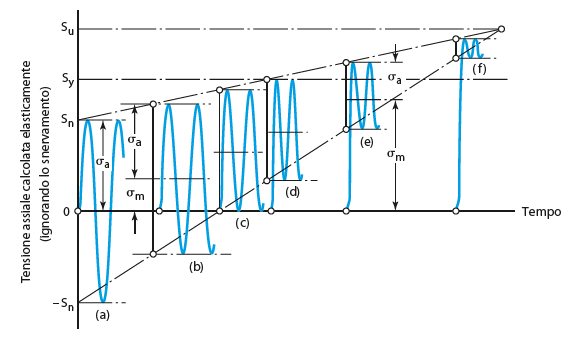
\includegraphics[width=1\linewidth]{figures/screenshot031}
		\label{fig:screenshot031}
	\end{figure}	
\end{adjustwidth}
\newpage
\section{Verifica a grippaggio secondo Block}
\begin{adjustwidth}{2in}{}	
	Questa verifica si vedrà per ora solo in termini qualitativi, le relazioni sperimentali secondo Block sono complesse e poco interessanti a fini didatti, tuttavia sono da tenere in considerazione perché influenzano la scelta del lubrificante. \newline 
	
	Il grippaggio avviene per condizioni di lubrificazione non ideali, ovvero a causa di elevate temperature locali, istantanee, il lubrificante raggiunge  una condizione di temperatura limite andando in sublimazione portando istantaneamente a contatto le superfici delle ruote dentate.
	
	Il contatto istantaneo avviene in punti caratterizzati da  strisciamento specifico non nullo e quindi si viene a creare un'adesione tra le parti con fusione, microsaldature e rottura istantanea di queste ultime. \newline 
	
	Queste raschiature finiscono anch'esse nel bagno dolio, portando a materiale interposto durante l'ingranamento e dunque ad un danneggiamento a catena dell'organo. \newline 
	
	Secondo la teoria di Block la temperatura che si manifesta nel contatto tra le dentature è legata ad effetti locali. 
	
	Sostanzialmente la temperatura che si instaura dell'inizio alla fine del contratto è dovuta ad una temperatura di \textit{bulk} intorno agli $80^\circ C$ che si instaura  a seguito dell'equilibrio termico tra lo smaltimento del calore del lubrificante e la creazione di calore dovuta all'attrito tra le parti, con l'aggiunta di una temperatura di \textit{flash} nel meato di lubrificante. 
	
	Quest'ultima è nulla nel centro di istantanea rotazione ed è non nulla nelle zone di contatto dov'è massimo lo scorrimento specifico questo reo di innalzamento delle temperature. 
	
	Se la somma 
	\[T_c = T_b+T_f\]
	Raggiunge un limite imposto dalla temperatura critica del lubrificante, allora si avrà sublimazione dello stesso e grippaggio locale. \newline 
	
	Valutare la temperatura di \textit{flash} è estremamente importante ma estremamente complesso perché dipende dagli scorrimenti specifici, dalle curvature delle superficie e da fattori prettamente legati alla lubrificazione. 
	
	L'obiettivo è quindi quello di tenere la temperatura \textit{flash} al di sotto della differenza tra la temperatura limite del lubrificante e quella \textit{bulk} di progetto. \newline 
	
	Alcune relazioni sperimentali traducono la temperatura \textit{flash} in un carico massimo transitante sul pezzo e quindi valutando che il carico sia sempre minore di quello limite che porta alla temperatura \textit{flash}.
	
	Individuata la temperatura \textit{flash} massima, si deve garantire che le caratteristiche del lubrificante siano sempre garantite. 
	\begin{figure}[H]
		\parbox{0.45\textwidth}{\centering
		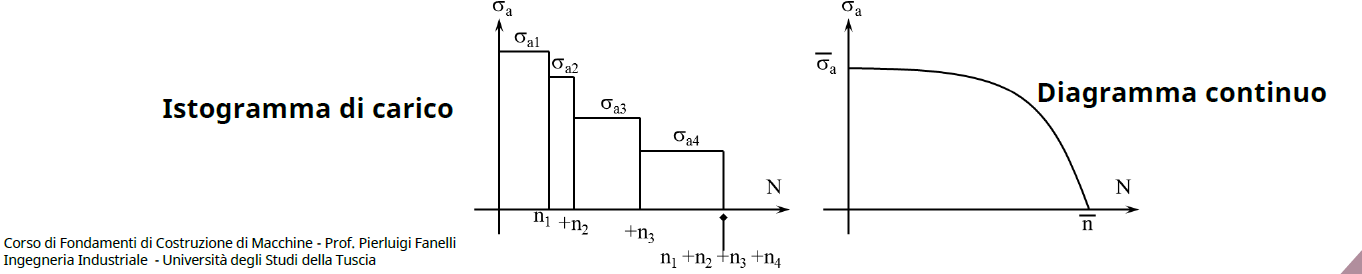
\includegraphics[width=1\linewidth]{figures/screenshot032}
		\label{fig:screenshot032}}
		\parbox{0.45\textwidth}{\centering
		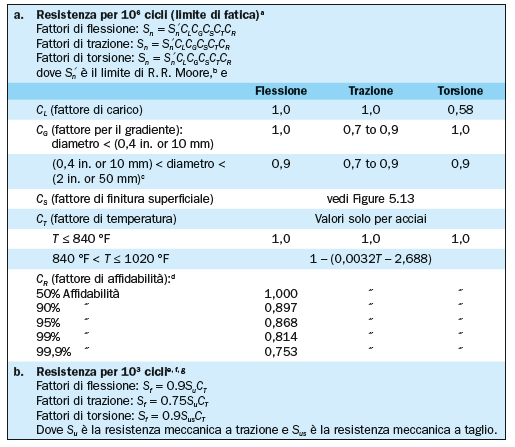
\includegraphics[width=1\linewidth]{figures/screenshot033}
		\label{fig:screenshot033}}
	\end{figure}
	
		
		
		





































\newpage
\textbf{{\LARGE NOTE}}
%	\vfill
%	\begin{tcolorbox}[height=4.5cm]
%		This box has a height of 4.5cm.
%	\end{tcolorbox}

%DA DECOMMENTARE PER AVERE LA VERSIONE STAMPABILE A DUE PAGINE 	
%	\newpage
%		\null
%		\vfill
%\begin{tcolorbox}[height=4.5cm]
%	This box has a height of 4.5cm.
%\end{tcolorbox}
%		
\end{adjustwidth}
\end{document}